\documentclass{standalone}

\usepackage{setspace}
\usepackage{times}
\usepackage{amsmath}
\usepackage{amssymb}
\usepackage{xparse}
\usepackage{ifthen}

\usepackage[dvipsnames]{xcolor}
\usepackage{tikz}
\usetikzlibrary{arrows,calc,patterns,patterns.meta}
\pgfdeclarelayer{background}
\pgfdeclarelayer{foreground}
\pgfsetlayers{background,main,foreground}

\usepackage{pgfplots}
\pgfplotsset{compat=1.15}

\definecolor{red}{HTML}{972e21}
\definecolor{yellow}{HTML}{ebb83f}
\definecolor{blue}{HTML}{5e7fbf}
\definecolor{green}{HTML}{5fd94e}
\renewcommand{\seriesdefault}{\bfdefault}
\renewcommand{\familydefault}{\sfdefault}

\begin{document}
   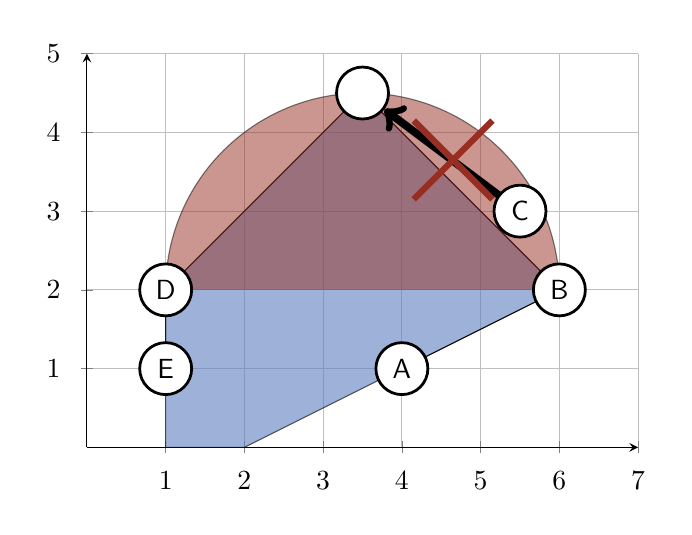
\begin{tikzpicture}[x=1cm,y=1cm,every node/.style={circle,inner sep=0pt,line width=1pt, minimum size = 0.66cm}]
        \begin{axis}[
            x=1.0cm,y=1.0cm,
            axis lines=middle,
            ymajorgrids=true,
            xmajorgrids=true,
            xmin=0,
            xmax=7,
            ymin=0,
            ymax=5,
            xtick={0.0,...,7.0},
            ytick={0.0,...,7.0},]  
            \begin{pgfonlayer}{foreground}
                \node[draw,fill=white] at (4cm,1cm) (a) {A};
                \node[draw,fill=white] at (6cm,2cm) (b) {B};
                \node[draw,fill=white] at (5.5cm,3cm) (c) {C};
                \node[draw,fill=white] at (1cm,2cm) (d) {D};
                \node[draw,fill=white] at (1cm,1cm) (e) {E};
                \node[draw,fill=white] at (3.5cm,4.5cm) (f) {};
            \end{pgfonlayer}
            \draw[fill=blue,opacity=0.6] (2cm,0cm) -- (b.center) -- (f.center) -- (d.center) -- (e.center) -- (1cm,0cm) -- cycle;
            \draw[-,line width=0.01cm,line join=round,black] (a.center) -- (b.center) -- (f.center) -- (d.center) -- (e.center);

            \begin{scope}
                \clip (10cm,5cm) rectangle (d.center);
                \draw[fill=red,opacity=0.5] (3.5cm,2cm) circle(2.5cm);
            \end{scope}

            \draw[->,line width=0.1cm,line join=round,black] (c.center) -- (f);
            \draw[red,line width=0.08cm] (4.15cm,3.15cm) -- (5.15cm,4.15cm);
            \draw[red,line width=0.08cm] (5.15cm,3.15cm) -- (4.15cm,4.15cm);

        \end{axis}

    \end{tikzpicture}
\end{document} 
